\documentclass{scrartcl}


%%% INCLUDE %%%

\usepackage[T1]{fontenc}
\usepackage[utf8]{inputenc}
\usepackage[french]{babel}
\usepackage{layout}
\usepackage{enumitem}
\usepackage{eurosym}
\usepackage{textcomp}
\usepackage{xstring}
\usepackage{array}
\usepackage{graphicx}

%%% MACRO %%%


% FIXME Prendre en compte les majuscule déjà présente
\makeatletter
\@ifpackageloaded{xstring}{
	\newcommand\smallcaps[1]{\StrLeft{#1}{1}\scriptsize\uppercase{\StrGobbleLeft{#1}{1}}\normalsize }
}{
	\newcommand\smallcaps[1]{\textsc{#1}}
}
\makeatother



%===============================================================================
% Définit un type de puce pour une liste. Si le pakage "pifont" est chargé, il 
% est utilisé, sinon on met un tiret.
\makeatletter
\@ifpackageloaded{pifont}{
	\newcommand\goodItemArrow[0]{\ding{226}}
}{
	\newcommand\goodItemArrow[0]{-}
}
\makeatother



%===============================================================================
% Item de liste avec spécification de la puce et paramètre écrit en gras.
\newcommand\functionality[1]{
	\item[\goodItemArrow] \textbf{#1}\\
}



%===============================================================================
% Commande \Euro indépendante des paquets chargés 
\makeatletter
\@ifpackageloaded{eurosym}{
	\newcommand\Euro[0]{\euro{}}
}{
	\@ifpackageloaded{textcomp}{
		\newcommand\Euro[0]{\texteuro}
	}{
		\newcommand\Euro[0]{Euro}
	}
}
\makeatother



%===============================================================================
% Accès à des variables dans le document. 
%\makeatletter
%\let\titleName\@title
%\let\subtitleName\@subtitle
%\let\authorName\@author
%\makeatother



% Titre de la section courante (que dans beamer)
%\secname 
% Titre de la sous-section courante (que dans beamer)
%\subsecname



% format.tex
% 
% author : Adrien Bisutti
% created : Mon, 26 Oct 2015 16:55:02 +0100
% modified : Mon, 26 Oct 2015 16:55:02 +0100
%

%\usepackage{soul}



%=== Section ===================================================================
% Grand chiffre romain, gras, souligné (FIXME souligné ne marche pas)
\makeatletter
\renewcommand\section{\@startsection {section}{1}{\z@}%
	{-3.5ex \@plus -1ex \@minus -.2ex}%
	{2.3ex \@plus.2ex}%
	{\Large\bfseries\sffamily\underline}}
\makeatother


\renewcommand{\thesection}{\Roman{section}}



%=== Sub-Section ===============================================================
% Chiffre arabe, gras, italique
\makeatletter
\renewcommand\section{\@startsection {section}{1}{\z@}%
	{-3.5ex \@plus -1ex \@minus -.2ex}%
	{2.3ex \@plus.2ex}%
	{\Large\bfseries\sffamily\itshape}}
\makeatother


\renewcommand{\thesubsection}{\arabic{subsection}}



%=== Paragraph =================================================================
% Interligne en dessous de 0.5
% TODO


%=== List ======================================================================
% Interligne en dessous de 1
% TODO


%=== Summary ===================================================================
% mettre des href avec http://www.xm1math.net/doculatex/structure.html
% TODO




%%% DATA %%%

%\title[Cahier des charges]{Surfaces de révolution discrètes}
\title{Surfaces de révolution discrètes}
\subtitle{Document de vision}
\author{
	Zied \bsc{Ben Othmane}\\
	Thomas \bsc{Benoist}\\
	Adrien \bsc{Bisutti}\\
	Lydie \bsc{Richaume}
}
%\institute{Université de Poitiers}


% TODO régler le layout
% TODO smallcaps correcte

\makeatletter
\let\titleName\@title
\let\subtitleName\@subtitle
\let\authorName\@author
\makeatother

%%% DOCUMENT %%%

\begin{document}


%===============================================================================
%	PAGE DE TITRE
%===============================================================================

\begin{titlepage}
	\vspace*{\stretch{1}}
	
	% --- Titre ---
	\begin{center}
		\fontsize{30}{36}\selectfont\bfseries
		\titleName\\
		\rule{6cm}{0.5pt} % trait horizontal de 6cm de long, 0.5pt d'épaisseur
	\end{center}
	
	% --- Sous-titre ---
	\begin{center}
		\LARGE
		\subtitleName
	\end{center}
	\vspace{1cm}
	
	% --- Auteurs ---
	\begin{center}
		\authorName
	\end{center}
	%\vfill
	% --- Logo ---
	%\begin{center}
	%	
\includegraphics[height=3cm]{../Images/logo_univ_poitiers.png}
	%	\hfill
	%	
\includegraphics[height=3cm]{../Images/logo-Xlim.png}
	%\end{center}
	%\vfill
	
	% --- Date ---
	\begin{center}
		\today
	\end{center}
\end{titlepage}
\newpage



%===============================================================================
%	SOMMAIRE
%===============================================================================

\tableofcontents
\newpage



%===============================================================================
%	ENVIRONNEMNT PROJET
%===============================================================================

\section{Environnement du projet}
	\subsection{Participants}
		\noindent
		Les Clients~:
			\begin{itemize}
				\item Éric \textsc{Andres} (Professeur et Directeur de département XLIM-SIC)
				\item Gaëlle \textsc{Largeteau-Skapin} (Maitre de Conférence, Géométrie discrète)
			\end{itemize}
		\medskip % FIXME
		
		\noindent
		Exemple d'utilisateur final~: Aurélie \textsc{Mourier} (Artiste)
		\medskip % FIXME
		
		\noindent
		Encadrant pédagogique~: Philippe \textsc{Meseure} (Professeur, Informatique graphique)
		\medskip % FIXME
		
		\noindent
		Composition de l'équipe~:
			\begin{itemize}
				\item Thomas \textsc{Benoist} (Chef de projet)
				\item Zied \textsc{Ben Othmane} (Responsable qualité)
				\item Adrien \textsc{Bisutti} (Responsable des riques)
				\item Lydie \textsc{Richaume} (Responsable des tâches)
			\end{itemize}
		\medskip % FIXME
	

% --- Contexte -----------------------------------------------------------------
	\subsection{Contexte}
		Éric \textsc{Andres} et Gaëlle \textsc{Largeteau-Skapin} ont conçu un nouvel algorithme pour modéliser des surfaces de révolution discrètes. Les résultats obtenus sont actuellement visualisés avec le logiciel Mathematica.
		%\begin{figure}[!h]
		%	\centering
		%	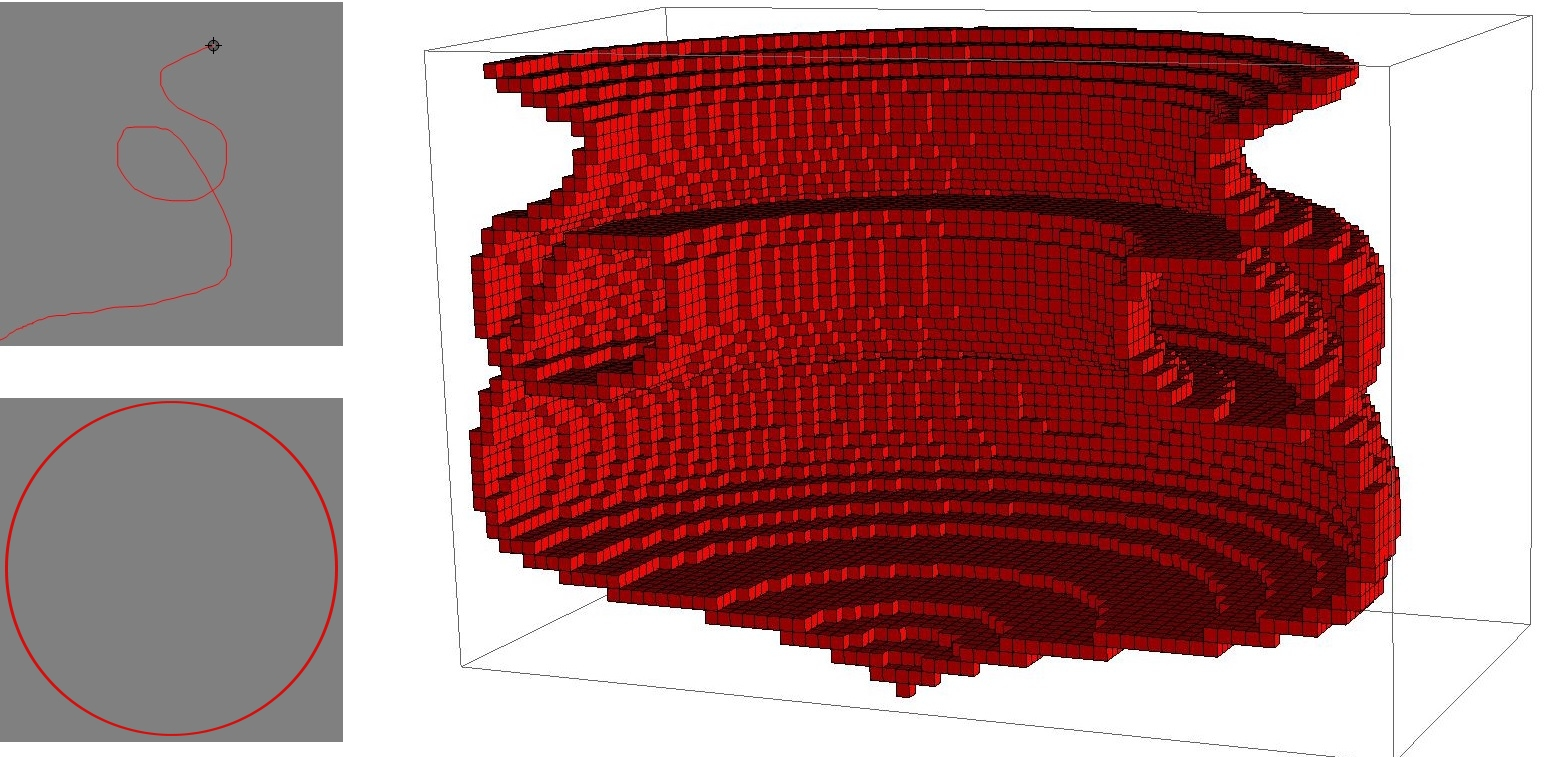
\includegraphics[height=3.8cm]{../Images/revolution2.jpg}
		%	\caption{Résultat de l'algorithme vu sur Mathématia}
		%\end{figure}
%		\begin{itemize}
%			\item[$\to$] Besoin de montrer les résultats et d'avoir un outil de création de surfaces de révolutions : but scientifique et artistique
%		\end{itemize}



%===============================================================================
%	OBJECTIF METIERS
%===============================================================================

\section{Objectifs métiers}


% --- Objectifs ----------------------------------------------------------------
	\subsection{Outils à développer}
		L'objectif de ce projet est de produire un outil de visualisation des surfaces générées par ce nouvel algorithme. Cet outil devra entre autre offrir la possibilité de réaliser les actions suivantes~:
		\begin{itemize}
			\item Visualiser les objets en 3D, en coupe
			\item Choisir les méridiennes et les courbes de révolution (listes de courbes prédéfinies, dessin à main levée, équation personnalisée)
	 		\item Exporter les objets obtenus (PNG, X3D, OBJ, STL, etc.)
		\end{itemize}
		
		Une première version de l'algorithme a déjà été fournie aux développeurs. Cet algorithme étant voué à évoluer, les prochaines versions pourront être intégrées au projet après négociation entre les partis et amendement du cahier des charges.

% --- Containtes----------------------------------------------------------------
% FIXME bon titre ?
	\subsection{Contraintes}
		L'application doit être disponible partout et par tous. En conséquence, l'outil fourni sera une application web disposant d'une interface simple et multi-langages. Cependant, cette simplicité d'interface ne doit en aucun cas biaiser les utilisateurs voulant disposer de fonctionnalités avancées.



%===============================================================================
%	OBJECTIFS TECHNIQUES
%===============================================================================

\section{Objectifs techniques}

% --- Techno envisagées --------------------------------------------------------
	\subsection{Technologies envisagées}
		L'application sera développée à l'aide des technologies disponibles avec HTML5 et notamment grâce aux canvas. Ces derniers seront exploités via l'API WebGL.
% XXX 
% Mathematica ?
% WebGL maitrisés par la plupart des membres de notre équipe
% Participation à un projet similaire


% --- Réutilisation Bifurcations -----------------------------------------------
	\subsection{Réutilisation de l'existant}
		L'application réutilisera le code d'une application existante ``Bifurcations''. Le moteur de rendu, la modélisation 3D et la base de l'interface pourront être réutilisés pour ce projet.
		%\begin{figure}[!h]
		%	\centering
		%	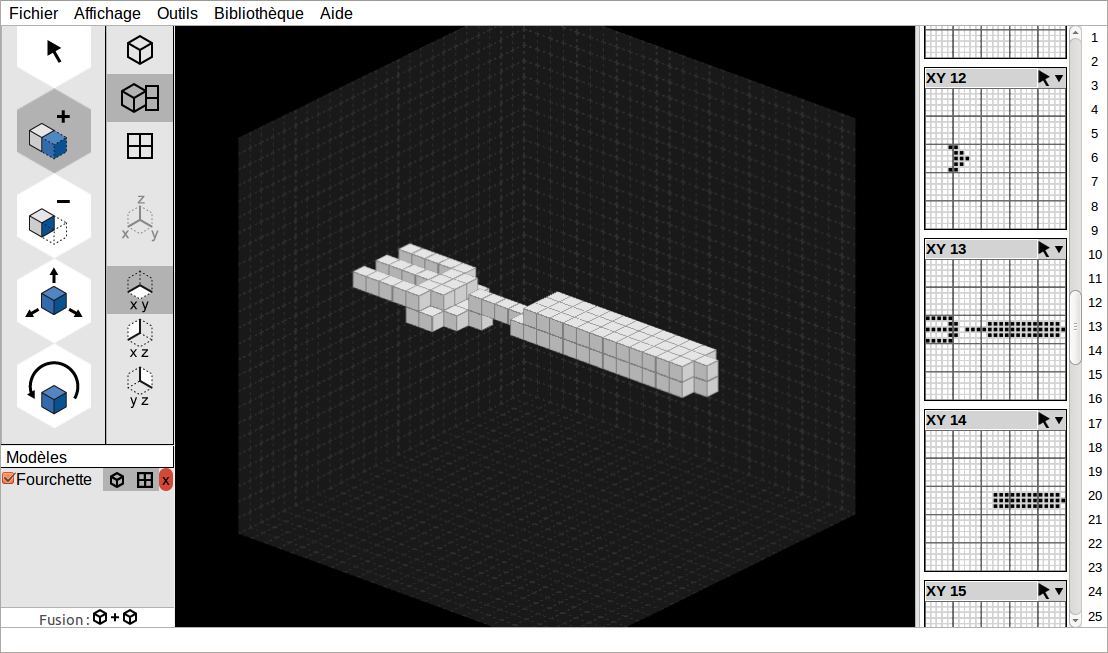
\includegraphics[width=12cm]{../Images/bifurcations_ihm.png}
		%	\caption{Interface de Bifurcations, application similaire.}
		%\end{figure}


% --- Gestion de projet --------------------------------------------------------
	\subsection{Gestion de projet}
		Le projet se déroulera suivant la méthode de développement en spirale. Cette méthode permettra de fournir une application minimale puis d'y ajouter de nouvelles fonctionnalités. Elle permettra également une organisation plus souple pour intégrer l'évolution des algorithmes ou de nouvelles demandes de la part des clients.
		Chaque fin de cycle aboutira à une nouvelle version de l'application, permettant ainsi de réaliser une validation incrémentale de celle-ci et de réorganiser le développement du projet en cas d'éventuelles erreurs.
% XXX Tâches importantes ?

\section{Présentation des résultats attendus}

	Le résultat que devra produire ce projet est une application web permettant de modéliser en 3D, de manière simple et rapide, une surface de révolution discrète.
% --- Cout ---------------------------------------------------------------------
	\subsection{Coûts}
		Le projet se déroulera sur dix  semaines et sera mené par une équipe de quatre jeunes ingénieurs. Aucune ressource particulière n'est requise. 
		En partant d'un coup de base de 3000 \Euro / mois pour un jeune ingénieur, le projet coutera donc 30 000 \Euro . En y ajoutant une marge de 30\% , le cout proposé aux clients est de 40 000\Euro
		
	\subsection{Délai}
		La rédaction du cahier des charges se fera sur la période précédant la réunion de lancement, du 19 au 30 Octobre.
		Le développement du projet prend place sur une période allant du 16 Novembre au 02 Mars (date de livraison des résultats). 


\section{Exemple de mise en oeuvre des résultats}

		\paragraph{Utilisation des paramètres simples}
			Un utilisateur pourra manipuler les courbes via des paramètres simples. Par exemple lorsqu'une courbe de révolution est un cercle, un des paramètres simple serait de modifier le diamètre.
			
		\paragraph{Utilisation des paramètres avancés}
			L'utilisation des paramètres avancés se traduit par la manipulation des coefficients de courbes, rentrer des équations pour les méridiennes/courbes de révolution.
			
		\paragraph{Tracer à main levée}
			Une des fonctionnalités importantes de l'application est que l'utilisateur pourra, s'il le souhaite, tracer ses méridiennes à main levée. Ce n'est cependant pas le cas pour les courbes de révolution.

\end{document}


